\documentclass[tikz]{standalone}
\usepackage{bm}
\usetikzlibrary{patterns}
\input{mathmacros}
\input{dissertationmacros}
\begin{document}
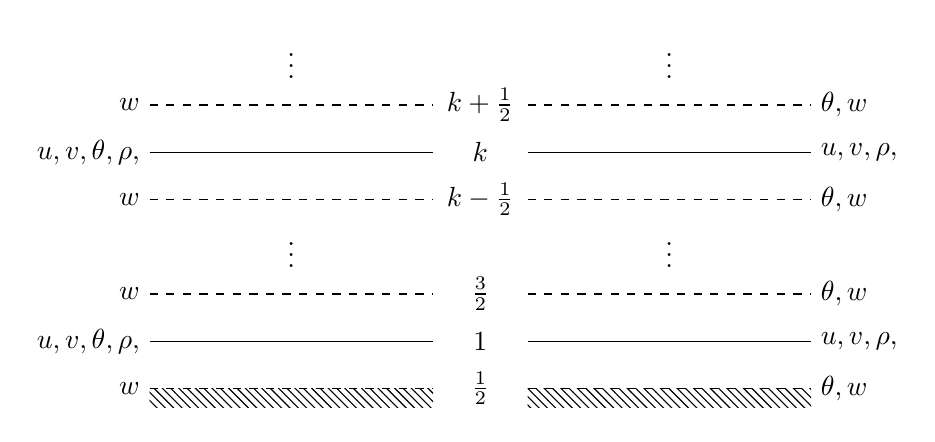
\begin{tikzpicture}[
  scale=0.6
]
\fill [pattern=north west lines] (0,0) rectangle (6,-0.4);
\fill [pattern=north west lines] (8,0) rectangle (14,-0.4);
\node at (7,0) {$\frac{1}{2}$};
\draw [dashed] (0,0) -- (6,0) node [at start, anchor=east] {$w$};
\draw [dashed] (8,0) -- (14,0) node [at end, anchor=west] {$\theta, w$};

\node at (7,1) {$1$};
\draw (0,1) -- (6,1) node [at start, anchor=east] {$u, v, \theta, \rho, \exner$};
\draw (8,1) -- (14,1) node [at end, anchor=west] {$u, v, \rho, \exner$};

\node at (7,2) {$\frac{3}{2}$};
\draw [dashed] (0,2) -- (6,2) node [at start, anchor=east] {$w$};
\draw [dashed] (8,2) -- (14,2) node [at end, anchor=west] {$\theta, w$};

\node at (3,3) {$\vdots$};
\node at (11,3) {$\vdots$};

\node at (7,4) {$k - \frac{1}{2}$};
\draw [dashed] (0,4) -- (6,4) node [at start, anchor=east] {$w$};
\draw [dashed] (8,4) -- (14,4) node [at end, anchor=west] {$\theta, w$};

\node at (7,5) {$k$};
\draw (0,5) -- (6,5) node [at start, anchor=east] {$u, v, \theta, \rho, \exner$};
\draw (8,5) -- (14,5) node [at end, anchor=west] {$u, v, \rho, \exner$};

\node at (7,6) {$k + \frac{1}{2}$};
\draw [dashed] (0,6) -- (6,6) node [at start, anchor=east] {$w$};
\draw [dashed] (8,6) -- (14,6) node [at end, anchor=west] {$\theta, w$};

\node at (3,7) {$\vdots$};
\node at (11,7) {$\vdots$};
\end{tikzpicture}
\end{document}
